\chapter{Differentiation and regularity}


\section{Differentiation of measures}

As an application, we define the conditional expectation of a random variable.
Recall from elementary probability theory that if $A$ is an event (which is not almost surely false) and $X$ is a random variable, then the conditional expectation of $X$ given $A$ is
\begin{equation}\label{conditional expectation event}
E(X|A) = \frac{E(1_{A}X)}{P(A)},
\end{equation}
the expected value of $X$ if we rescale $A$ to be the entire probability space.
However, in probability theory, one often needs to discuss the conditional expectation of $X$ with respect to not just an event, but an entire $\sigma$-algebra of events.
More precisely, let $\mathcal F$ be a $\sigma$-algebra.
If $A \in \mathcal F$ and we define $E(X|A)$ by (\ref{conditional expectation event}), then we forget everything $X$ except its mean on $A$.
The conditional expectation of $X$ on $\mathcal F$, by definition, will be a random variable that only remembers the conditional expectations of $X$ with respect to every event in $\mathcal F$.

\begin{definition}
Let $(\Omega, \Sigma, P)$ be a probability space, $\mathcal F \subseteq \Sigma$ a $\sigma$-algebra, and $X \in L^{1}(\Omega \to \RR)$ a random variable.
The \dfn{conditional expectation} of $X$ given $\mathcal F$ is a measurable function
\[E(X|\mathcal F): (\Omega, \mathcal F) \to \RR\]
such that
\[E(1_{A} E(X|\mathcal F)) = E(1_{A} X)\]
whenever $A \in \mathcal F$.
\end{definition}

\begin{example}
A \dfn{measurable partition} of $\Omega$ is a set of mutually exclusive events $A_{i}$ such that $\bigcup_{i} A_{i} = \Omega$.
If $(A_{i})$ is a measurable partition and $\mathcal F$ is the smallest $\sigma$-algebra containing every $A_{i}$, then $E(X|\mathcal F)$ is constant on each $A_{i}$, namely
\[E(X|\mathcal F)|A_{i} = E(1_{A_{i}} X)\]
is the mean of $X$ on $A_{i}$.
\end{example}

\begin{corollary}
Let $(\Omega, \Sigma, P)$ be a probability space, $\mathcal F \subseteq \Sigma$ a $\sigma$-algebra, and $X \in L^{1}(\Omega \to \RR)$ a random variable.
The conditional expectation $E(X|\mathcal F)$ is well-defined in the sense that it exists, and if $Y$ is also a conditional expectation, then $E(X|\mathcal F) = Y$ almost surely.
\end{corollary}
\begin{proof}
Let $\mu$ be the measure
\[\mu(A) = E(1_{A} X)\]
defined for $A \in \mathcal F$.
Then $\mu$ is absolutely continuous with respect to $P$, so it has a Radon-Nikodym derivative; we set
\[E(X|\mathcal F) = \frac{d\mu}{dP}.\]
Then
\[E(1_{A} E(X|\mathcal F)) = \int_{A} \frac{d\mu}{dP} ~dP = \int_{A} ~d\mu = \mu(A) = E(1_{A} X)\]
as desired.

For the uniqueness, assume $Y$ is also a conditional expectation and let $A$ be the event that $Y \neq E(X|\mathcal F)$.
Then $A \in \mathcal F$ so
\[E(1_{A}|Y - E(X|\mathcal F)|) = E(1_{A}|X - X|) = 0.\]
But $|Y - E(X|\mathcal F)| > 0$ on $A$ so this implies $E(1_{A}) = 0$, thus $A$ is almost surely false.
\end{proof}

\begin{exercise}
Let $X \in L^{1}$ be a random variable and $\mathcal F$ a $\sigma$-algebra. Show that if the pullback $\sigma$-algebra induced by $X$ is independent of $\mathcal F$ then
\[E(X|\mathcal F) = E(X).\]
Show that
\[E(E(X|\mathcal F)) = E(X).\]
Show that if $X$ is $\mathcal F$-measurable then $E(X|\mathcal F) = X$.
\end{exercise}

\begin{exercise}
Verify that the monotone and dominated convergence theorems, and Fatou lemma, are valid when $EX_{n}$ is replaced with $E(X_{n}|\mathcal F)$, $\mathcal F$ a $\sigma$-algebra.
\end{exercise}

\section{Existence of Radon measures}

\section{Differentation of vector-valued functions}

\section{Vitali covers and maximal inequalities}
We want to prove the Lebesgue differentiation theorem -- Lebesgue's generalization of the fundamental theorem of calculus to functions that are just in $L^1_{loc}$.
Before we do so, we will need some combinatorial facts about open balls in metric spaces, and a certain kind of inequality called a maximal inequality.
Both turn out to be of independent interest.

\begin{subsec}
Let us recall some terminology about metric spaces.
In a metric space $X = (X, d)$, a \dfn{ball} $B$ is any set of the form $B(x, r) = \{y \in X: d(x, y) < r\}$, where $x \in X$ and $r > 0$.
If $B$ is a ball, say $B = B(x, r)$, we let $kB$ denote the \dfn{dilated ball} $kB = B(x, kr)$, and put $\rad B = r$.
\end{subsec}

\begin{subsec}
Our first task is to solve \dfn{Vitali's covering problem}: given a set $\mathcal B$ of balls, we will find a smaller subset which is disjoint but, after dilation by a factor of $3 + \varepsilon$, covers as much of the metric space as $\mathcal B$ did.
To do this, we first treat the case that $\mathcal B$ is a finite set.
After treating the case of finite sets, we use Zorn's lemma to generalize to the case of infinite sets.
\end{subsec}

\begin{figure}\label{Vitali Figure1}
\caption{The state of the greedy algorithm after the zeroth, first, third, and final (sixth) stages. The blue balls have not yet been added to $\mathcal B_{0}$, the green ball has just been chosen to be added to $\mathcal B_{0}$, and the red balls are already in $\mathcal B_{0}$. At each stage the algorithm chooses the largest ball that does not intersect any red balls to add to $\mathcal B_{0}$. After the final phase, this is impossible, and the $3$-dilates of the red balls cover every blue ball.}
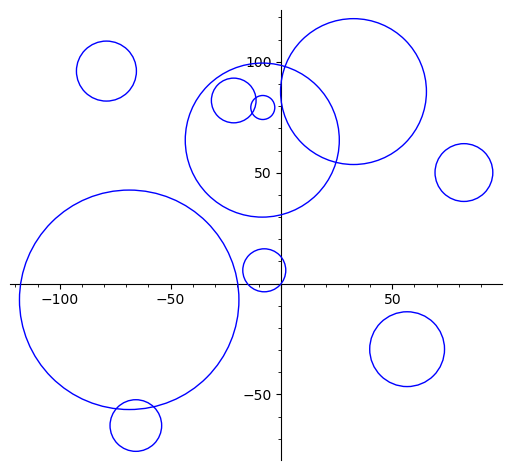
\includegraphics[width=.48\textwidth]{graphics/Vitali11}\hfill
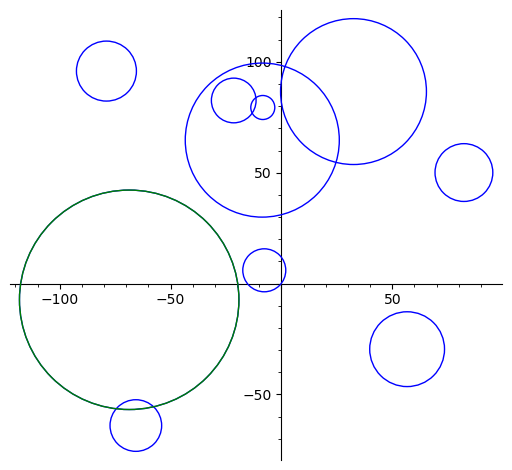
\includegraphics[width=.48\textwidth]{graphics/Vitali12}\\
[\smallskipamount]\\[\smallskipamount]
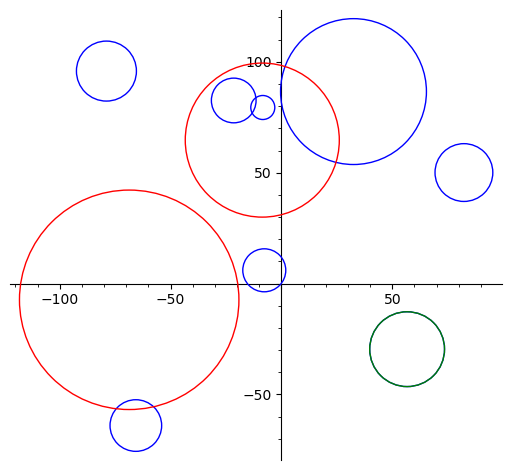
\includegraphics[width=.48\textwidth]{graphics/Vitali13}\hfill
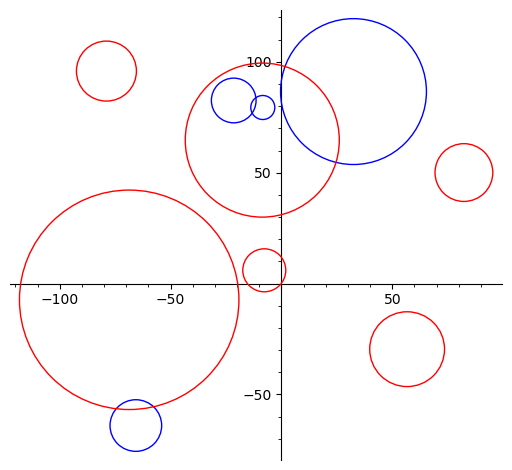
\includegraphics[width=.48\textwidth]{graphics/Vitali14}
\end{figure}

\begin{subsec}
The finite case of Vitali's covering problem, Theorem \ref{finite Vitali problem}, is solved by a \dfn{greedy algorithm}: we want our to cover as much of the metric space as possible, so at every step of the construction, we pick the ball which covers as much of the metric space as possible. See Figure~\ref{Vitali Figure1}.
Greedy algorithms are frequently useful in applications, especially software design.
This is why we prove the finite case separately -- the reader who is not interested in greedy algorithms can skip Theorem \ref{finite Vitali problem} and only treat the infinite case.
\end{subsec}

\begin{figure}
\label{Vitali Figure2}
\caption{The ball $B$ in red meets the small ball $B_{0}$ in green, and hence is contained in its dilate, the large ball in green.
Here $\rad B_{0} = 1.1$ while $\rad B = 1$, so the red point is nearly $2$ units away from the blue point, and $3.1 < 3.3$ units away from the green point.}
\centering 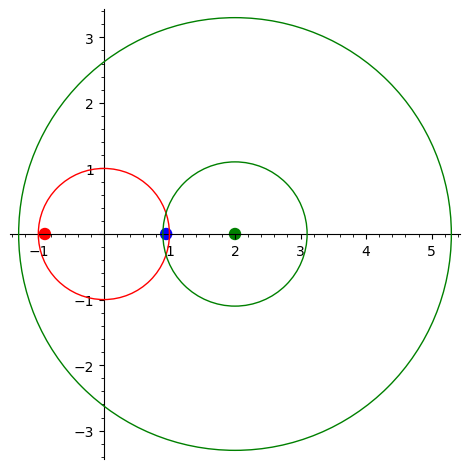
\includegraphics[width=0.5\textwidth]{graphics/Vitali2}
\end{figure}

\begin{theorem}[solving Vitali's covering problem, finite case]\label{finite Vitali problem}
Let $X$ be a metric space and let $\mathcal B$ be a finite set of balls in $X$. Then there is a subset $\mathcal B_{0}$ of $\mathcal B$ consisting of disjoint balls such that
\[\bigcup_{B \in \mathcal B} B \subseteq \bigcup_{B_{0} \in \mathcal B_{0}} 3B_{0}.\]
\end{theorem}
\begin{proof}
We proceed by induction.
If $\mathcal B$ is empty then there is nothing to prove.
Otherwise, suppose that we are given disjoint balls $B_1, \dots, B_n$.
If there are balls in $\mathcal B$ which are disjoint from $\bigcup_{j \leq n} B_j$, let $B_{n+1}$ be one such ball with the largest possible radius.
If no such ball exists, let $\mathcal B_0 = \{B_1, \dots, B_n\}$.

Now let $Y = \bigcup_{B_{0} \in \mathcal B_{0}} 3B_{0}$ and let $B \in \mathcal B$.
It remains to show $B \subseteq Y$. If $B = B_j$ for some $j \in \{1, \dots, n\}$ this is clear.
Otherwise, there exists $j \in \{1, \dots, n\}$ such that $B \cap B_j$ is nonempty and $\rad B \leq \rad B_j$ -- if not, we would have chosen $B$ at some stage of the construction of $\mathcal B_{0}$.
If $x \in B$, $y \in B \cap B_j$, and $z$ is the center of $B_j$, then $d(y, z) \leq \rad B_j$ and $d(x, y) \leq 2\rad B \leq 2\rad B_j$, as in Figure \ref{Vitali Figure2}.
So
\[d(x, z) \leq d(x, y) + d(y, z) \leq 3 \rad B_j\]
whence $x \in B_j \subseteq Y$.
\end{proof}

\begin{lemma}
Let $X$ be a set, and let $\mathcal D$ be a set of subsets of $X$.
Then there exists a disjoint subset $\mathcal C$ of $\mathcal D$ which is maximal in the sense that if $\mathcal C'$ contains $\mathcal C$, then there are $C,C' \in \mathcal C'$ with $C \cap C' \neq \emptyset$.
Furthermore, if $D \in \mathcal D$ then there is $C \in \mathcal C$ such that $D \cap C$ is nonempty.
\end{lemma}
\begin{proof}
We proceed by Zorn's lemma.
Let $\PP$ be the set of all disjoint subsets of $\mathcal D$; since $\emptyset \in \PP$, $\PP \neq \emptyset$.
Let $\mathbb K$ be a chain in $\PP$.
Then if $K, K' \in \bigcup \mathbb K$, there is already a $\mathcal K \in \mathbb K$ such that $K, K' \in \mathcal K \in \PP$.
So $K,K'$ are disjoint, and $\bigcup \mathbb K \in \PP$.

If there is $D \in \mathcal D$ which misses every set in $\mathcal C$, we could add $D$ to $\mathcal C$ without breaking disjointness.
But this contradicts the fact that Zorn's lemma always returns a maximal set.
\end{proof}

\begin{theorem}[solving Vitali's covering problem, infinite case]
Let $X$ be a metric space and let $\mathcal B$ be a set of balls in $X$. Let
\[R(\mathcal B) = \sup_{B \in \mathcal B} \rad B\]
be the supremum of radii of the balls in $\mathcal B$. If $R(\mathcal B) < \infty$ then for every sufficiently small $\varepsilon > 0$ there is a subset $\mathcal B_{0}(\varepsilon)$ of $\mathcal B$ consisting of disjoint balls such that
\begin{equation}\label{Vitali formula}
\bigcup_{B \in \mathcal B} B \subseteq \bigcup_{B_{0} \in \mathcal B_{0}(\varepsilon)} (3 + \varepsilon)B_{0}.
\end{equation}
\end{theorem}
\begin{proof}
If $\varepsilon$ is small then there exists $1 < \delta < 2$ so small that $1 + 2\delta < 3 + \varepsilon$.
Write
\[\mathcal B = \bigcup_{n \geq 1} \mathcal B^n\]
where $\mathcal B^n$ consists of balls whose radius is in $(\delta^{-n-1}R(\mathcal B), \delta^{-n}R(\mathcal B)]$.
Let $\mathcal C^0$ be a maximal disjoint subset of $\mathcal B^0$.
Suppose that we are given $\mathcal C^0, \dots, \mathcal C^{n - 1}$.
Let $\mathcal D^{n}$ be the set of all $B \in \mathcal B^{n}$ which are disjoint from every ball in $\mathcal C^{j}$ for every $j < n$, and let $\mathcal C^{n}$ be a maximal disjoint subset of $\mathcal C^{n}$.
Once this process is complete, let $\mathcal B_{0}(\varepsilon) = \bigcup_{n \geq 1} \mathcal C^{n}$.

We now must show (\ref{Vitali formula}).
So let $B \in \mathcal B$, in which case we can find $n$ such that $B \in \mathcal B^{n}$.

We claim that there is a ball $C \in \mathcal C^{j}$ for some $j \leq n$ such that $B \cap C$ is nonempty.
If $n > 0$ and $B \notin \mathcal D^{n}$, then there is a ball in $\mathcal C^{j}$ for some $j < n$ which meets $B$.
Otherwise, $B \in \mathcal D^{n}$ or $n = 0$, so $B$ meets a ball in the maximal disjoint set $\mathcal C^{n}$.
This proves the claim.

In particular,
\[\rad C > \delta^{-n-1}R(\mathcal B).\]
But $\rad B \leq \delta^{-n}R(\mathcal B)$, so $\rad B < \delta\rad C$. Now if $x \in B$, $y \in B \cap C$, and $z$ is the center of $C$, we have
\[d(x, z) \leq d(x, y) + d(y, z) \leq 2\delta \rad C + \rad C < (3 + \varepsilon) \rad C\]
which proves (\ref{Vitali formula}).
\end{proof}

\begin{subsec}
Now we turn to the most important application of Vitali coverings: the Hardy-Littlewood maximal inequality.
This inequality controls the Lebesgue measure of the set on which a function $f \in L^1(\RR^d)$ is allowed to be ``large on average".
The point of this inequality is that it will allow us to prove almost-everywhere convergence of certain sequences that already converge in $L^1$, but at a price: we will have no control on the rate at which the sequence converges, and in general it will converge arbitrarily slowly.
\end{subsec}

\begin{definition}
Let $V$ be a Banach space.
The \dfn{Hardy-Littlewood maximal function} of a function $f \in L^1_{loc}(\RR^d, V)$ is
$$Mf(x) = \sup_{r > 0} \frac{1}{|B(x, r)|} \int_{B(x, r)} ||f(y)||_V ~dy$$
where $|\cdot|$ is Lebesgue measure.
\end{definition}

\begin{theorem}[weaktype Hardy-Littlewood maximal inequality]
Let $d \geq 1$, $V$ a Banach space, and $f \in L^{1}(\RR^{d})$. Let $|\cdot|$ denote Lebesgue measure. Then for every $\lambda > 0$,
\[\mu(\{Mf > \lambda\}) \leq 3^{d} \frac{||f||_{L^{1}(\RR^{d} \to V)}}{\lambda}.\]
\end{theorem}
\begin{proof}
Let $\varepsilon > 0$.
If $Mf(x) > \lambda$ then there is a ball $B$ centered at $x$ such that
$$\int_B ||f(y)||_V ~dy > \lambda |B|.$$
Let $\mathcal B(\varepsilon)$ be the set of all such balls of radius $\leq 1/\varepsilon$.
By Vitali's theorem we can find a countable set of disjoint balls $\mathcal B_0(\varepsilon) \subseteq \mathcal B(\varepsilon)$ such that $\bigcup_{B_{0} \in \mathcal B_{0}(\varepsilon)} (3 + \varepsilon)B_{0}$ covers $\{Mf > \lambda\}$.
That is,
$$\sum_{B_{0} \in \mathcal B_{0}(\varepsilon)} |(3 + \varepsilon) B_{0}| = (3 + \varepsilon)^d \sum_{B_{0} \in \mathcal B_{0}(\varepsilon)} |B_{0}| \leq \frac{(3 + \varepsilon)^d}{\lambda} \sum_{B_{0} \in \mathcal B_{0}(\varepsilon)} ||f(y)||_V ~dy.$$
We now use the fact that
$$\sum_{B_{0} \in \mathcal B_{0}(\varepsilon)} ||f(y)||_V ~dy \leq ||f||_{L^1}$$
since $\mathcal B_{0}(\varepsilon)$ is disjoint.
We also have
$$|\{Mf > \lambda\}| \leq \sup_{\varepsilon > 0} \sum_{B_{0} \in \mathcal B_{0}(\varepsilon)} |(3 + \varepsilon) B_{0}|$$
since if $Mf(x) > \lambda$ then the ball $B$ centered at $x$ such that
$$\int_B ||f(y)||_V ~dy > \lambda |B|$$
satisfies $\rad B \leq 1/\varepsilon$ for some $\varepsilon$.
Summing up we have
$$|\{Mf > \lambda\}| \leq (3 + \varepsilon)^{d} \frac{||f||_{L^{1}(\RR^{d})}}{\lambda}$$
for every $\varepsilon > 0$ and hence also for $\varepsilon = 0$.
\end{proof}

\begin{exercise}
Show that the constants in Vitali's theorem are optimal -- we cannot replace $3$ by $3 - \delta$ for any $\delta$ in the finite case, nor can we replace $3 + \varepsilon$ with $3$ in the infinite case.
\end{exercise}

\begin{exercise}
Show that in a separable metric space, the set $\mathcal B_0$ of balls returned by Vitali's theorem is always countable.
But show that there is a metric space and a set of balls $\mathcal B$ for which $\mathcal B_0$ is uncountable.
\end{exercise}

\begin{exercise}
Show that there is a counterexample to Vitali's theorem when $R(\mathcal B)$ is infinite.
\end{exercise}

\begin{exercise}
Implement Vitali's greedy algorithm in Sage for the case $X = \QQ^2$, and use it to solve Vitali's covering problem with $\mathcal B$ given by \url{https://clopen-analysis.github.io/sage/vitali.sage}. TODO: Make this dataset!
What is the time complexity of Vitali's greedy algorithm, and can you optimize it?
\end{exercise}

\begin{exercise}[Vitali]
A \dfn{fine cover} $\mathcal F$ of a metric space $X$ is an open cover of $X$ such that for every $x \in X$ and ball $B \ni x$, there is $F \in \mathcal F$ such that $x \in F \subseteq B$.
Show that for every bounded Lebesgue measurable subset $X$ of $\RR^d$, fine cover $\mathcal F$ of $X$ by balls, and $\varepsilon > 0$, there is a countable disjoint subset $\mathcal F_0$ which covers almost all of $X$ and
$$\left|\bigcup_{F_{0} \in \mathcal F_{0}} F_{0}\right| \leq |X| + \varepsilon.$$
\end{exercise}

\begin{exercise}
Let $f \in L^{1}(\RR^{d})$.
Show that if $Mf \in L^{1}(\RR^{d})$ then $f = 0$.
It may help to first try this when $f$ has compact support.
\end{exercise}

\section{The Lebesgue differentation theorem}
We are ready to prove Lebesgue's vast generalization of the fundamental theorem of calculus.

\begin{definition}
Let $X$ be a metric space and let $x \in X$.
If $F$ is a function defined on balls, we write
$$\lim_{B \to x} F(B) = L$$
to mean that for every $\varepsilon > 0$, there is a ball $B \ni x$ such that for every ball $x \in B' \subseteq B$, $|F(B) - L| < \varepsilon$.
We define
$$\limsup_{B \to x} F(B) = L$$
if $L$ is the supremum over all sequences of balls $B_j \ni x$ with $\rad B_j \to 0$ of the quantity $F(B_j)$, and similarly define the limit inferior.
\end{definition}

\begin{subsec}
If $F$ is a function defined on balls, then the limit of $F$ in the above sense exists iff its limit superior and limit inferior are equal.
Furthermore, if the limit exists, it is unique.
The proofs are the same as for any other definition of limit, and thus omitted.
\end{subsec}

\begin{subsec}
The reader who is familiar with convergence of nets (Definition~\ref{convergence of nets}) will recognize that the above limit definition is no more than convergence of nets, where the set of open balls containing $x$ is given the structure of a directed set by writing $B' \geq B$ to mean $B \subseteq B'$.
Indeed, $\sup(B_1, \dots, B_n) = B_1 \cap B_2 \cap \cdots B_n$, so the set of open balls containing $x$ is directed.
\end{subsec}

\begin{subsec}
Now recall the notion of an indefinite integral. If $f \in L^1(X \to \CC)$ we define the measure
$$\nu(E) = \int_E f ~d\mu$$
to be the indefinite integral of $f$. If $X = \RR$, $\mu$ is Lebesgue measure, and $E_x = (-\infty, x]$ then we have
$$\nu(E_x) = \int_{-\infty}^x f(y) ~dy$$
so that the indefinite integral generalizes the familiar notion from calculus.
Indeed, if $f$ is continuous, then the fundamental theorem of calculus says that
$$\frac{d}{dx}~\nu(E_x) = f(x).$$
Expanding out the definition of the derivative, we conclude that the fundamental theorem of calculus is equivalent to the statement
$$\lim_{h \to 0} \frac{1}{h} \int_{x}^{x + h} f(y) ~dy = f(x)$$
which can be written more abstractly as
\begin{equation}
\label{Lebesgue point}
\lim_{B \to x} \frac{1}{|B|} \int_B f(y) ~dy = f(x)
\end{equation}
where $|B|$ is the volume of $B$.
\end{subsec}

\begin{definition}
Let $f \in L^1_{loc}(\RR^d)$.
We say that $x$ is a \dfn{Lebesgue point} of $f$ if (\ref{Lebesgue point}) holds.
\end{definition}

\begin{subsec}
Thus, the fundamental theorem of calculus says that if $f$ is continuous on $\RR$, then every real number is a Lebesgue point of $f$.
We will need that this is true for functions on $\RR^d$ as well.
\end{subsec}

\begin{lemma}\label{fundamental continuous theorem}
Every point of $\RR^d$ is a Lebesgue point of every continuous function on $\RR^d$.
\end{lemma}
\begin{proof}
We have already argued that this is true if $d = 1$, by the fundamental theorem of calculus.

Let $f$ be a continuous function and $\varepsilon > 0$.
We will show that $f$ is continuous at $0$; after translating, the same argument applies anywhere.

We first show the result when $B$ is centered on $0$.
Let $r = \rad B$, and write in polar coordinates
$$\frac{1}{|B|} \int_B f(y) ~dy = \frac{1}{r^d} \frac{1}{\alpha_{d - 1}} \int_0^r \int_{S^{d - 1}} f(s, \omega) ~d\omega ~ds$$
where $S^{d-1}$ is the unit sphere in $\RR^d$ and $\alpha_{d - 1}$ is its surface area (and $d\omega$ is with respect to spherical measure).
Taking the limit as $r \to 0$, we get
$$\lim_{r \to 0}\frac{1}{r^d} \frac{1}{\alpha_{d - 1}} \int_0^r \int_{S^{d - 1}} f(s, \omega) ~d\omega ~ds = \frac{1}{\alpha_{d - 1}} \int_{S^{d - 1}} f(0) ~d\omega = f(0)$$
by this result with $d = 1$.

Now we prove it for arbitrary balls.
We pass to a subsequence $(B_j)$ along which the limit exists. Each ball in the subsequence contains a ball which is centered on $0$, so the definition of the limit implies that
$$\lim_{j \to \infty} \frac{1}{|B_j|} \int_{B_j} f(y) ~dy = f(x)$$
as desired.
\end{proof}

\begin{theorem}[Lebesgue differentiation theorem]
Let $f \in L^1_{loc}(\RR^d \to \CC)$. Then almost every $x \in \RR^d$ is a Lebesgue point of $x$.
\end{theorem}
\begin{proof}
Let
$$F(B) = \frac{1}{|B|} \int_B f(y) ~dy.$$
We want to show that
\begin{equation}\label{LDT limit}
\lim_{B \to x} F(B) = f(x)
\end{equation}
almost everywhere.

First we show that (\ref{LDT limit}) holds along a subsequence of balls.
To do that, we fix a compact set $K \subset \RR^d$ and prove that (\ref{LDT limit}) holds in $L^1(K)$.
In fact, by Lemma~\ref{fundamental continuous theorem}, (\ref{LDT limit}) holds in the topology of $L^1(K)$ for a dense subset of $L^1(K)$, namely the continuous functions on $K$, so it holds for all of $L^1(K)$.
After taking a subsequence we conclude that (\ref{LDT limit}) holds almost everywhere in $K$, but $K$ was arbitrary, so (\ref{LDT limit}) holds along a subsequence almost everywhere.

Let $\delta > 0$; we write $f = f_\delta + (f - f_\delta)$ where $||f_\delta||_{L^1} < \delta$ and $f - f_\delta$ is continuous.
Let
$$g(x) = \limsup_{B \to x} F(B) - \liminf_{B \to x} F(B)$$
and let $g_\delta$ be the analogous function for $f_\delta$, $h_\delta$ the analogous function for $f - f_\delta$.
Then $h_\delta = 0$ by Lemma~\ref{fundamental continuous theorem}, and
$$|g| \leq |h_\delta| + |g_\delta| = |g_\delta| \leq 2Mg_\delta.$$
By the Hardy-Littlewood maximal inequality, it follows that
$$|\{|g| > \varepsilon\}| \leq 6^d\frac{\delta}{\varepsilon}$$
where $|E|$ denotes the Lebesgue measure of the measurable set $E$.
If we take $\delta < \varepsilon^2$ we conclude that
$$|\{|g| > \varepsilon\}| < 6^d\varepsilon$$
or in other words $g = 0$ almost everywhere. In particular the limit of $F(B)$ as $B \to x$ must exist for almost every $x$.

But we know that (\ref{LDT limit}) holds along a subsequence almost everywhere.
So, since the limit exists almost everywhere along the mother sequence, (\ref{LDT limit}) holds almost everywhere along the mother sequence.
\end{proof}

\begin{subsec}
The above argument was essentially standard.
We first show convergence of a sequence $(h_n)$ almost everywhere along a subsequence to a quantity $h$, and then apply the Hardy-Littlewood maximal inequality to the quantity
$$\limsup_{n \to \infty} h_n - \liminf_{n \to \infty} h_n$$
to deduce that in fact $(h_n)$ has a limit, which hence must be $h$.
In general, related inequalities to the Hardy-Littlewood maximal inequalities, known generally as maximal inequalities, are powerful tools for proving almost everywhere convergence.
\end{subsec}

\begin{definition}
Let $E \subseteq \RR^d$ be a Lebesgue measurable set and let $|\cdot|$ denote Lebesgue measure.
The quantity
$$\delta_E(x) = \lim_{B \to x} \frac{|E \cap B|}{|B|}$$
is called the \dfn{density} of $E$ at $x$. The set $\{0 < \delta_E < 1\}$ is called the \dfn{measure-theoretic boundary} of $E$.
\end{definition}

\begin{theorem}[Lebesgue density theorem]
The measure-theoretic boundary of every Lebesgue measurable set is null.
\end{theorem}
\begin{proof}
Apply the Lebesgue differentiation theorem to the function $1_E$ where $E$ is Lebesgue measurable.
Since that function is either $0$ or $1$, its averages over balls must limit to $0$ or $1$ almost everywhere.
\end{proof}

\begin{subsec}
Another important consequence of the Lebesgue differentiation theorem is a test to determine when functions are differentiable.
\end{subsec}

\begin{definition}
Let $X$ be a metric space and $f: X \to B$ a function. The \dfn{Lipschitz seminorm} of $f$ is
$$[f] = \sup_{x \neq y} \frac{|f(x) - f(y)|}{d(x, y)}.$$
A \dfn{Lipschitz function} is a function whose Lipschitz seminorm is finite.
\end{definition}

\begin{subsec}
One can show that every Lipschitz function is continuous. The space of Lipschitz functions on a compact metric space $K$ is equipped with the supremum norm plus the Lipschitz seminorm; that is,
$$||f|| = \sup_{x \in K} |f(x)| + \sup_{x \neq y} \frac{|f(x) - f(y)|}{d(x, y)}.$$
\end{subsec}

\begin{theorem}[Rademacher differentation theorem]
Every Lipschitz function $f: \RR \to \CC$ is differentiable almost everywhere,
$$||f'||_{L^\infty} \leq [f],$$
and one has
\begin{equation}\label{Rademacher FTC}
f(y) = f(x) + \int_x^y f'(z) ~dz
\end{equation}
whenever $x < y$.
\end{theorem}
\begin{proof}
By breaking up $f$ into real and imaginary parts we may assume that $f$ is real-valued.
Since $f$ is continuous, we may let $\mu$ be the Stieltjes measure arising from $f$.

We first claim that $\mu$ is absolutely continuous with respect to Lebesgue measure.
Indeed, if $E \subset \RR$ is a Lebesgue null set, then for every $\varepsilon > 0$ there exist half-open intervals $([a_j, b_j))_j$ which cover $E$ such that $\sum_j b_j - a_j < \varepsilon$.
But then
$$||\mu||(E) \leq \sum_j |f(b_j) - f(a_j)| \leq [f] \sum_j b_j - a_j < [f]\varepsilon$$
so $E$ is also $\mu$-null.

So by the Radon-Nikod\'ym theorem there is a function $f' \in L^1_{loc}(\RR)$ such that for every Borel set $E$,
$$\mu(E) = \int_E f'(x) ~dx.$$
In particular, if $E = [a, b]$ we deduce that (\ref{Rademacher FTC}) holds.

We must show that $f'$ is the honest derivative of $f$ almost everywhere; in fact,
$$\lim_{h \to 0} \frac{f(x + h) - f(x)}{h} = \lim_{h \to 0} \frac{1}{h} \int_{x}^{x + h} f'(y) ~dy = \lim_{B \to x} \frac{1}{|B|} \int_B f'(y) ~dy = f'(x)$$
almost everywhere by the Lebesgue differentiation theorem.
Since this is the usual definition of the derivative, we see that the two different possible values of $f'$ agree almost everywhere.

Finally we bound for almost every $x$
$$|f'(x)| = \lim_{h \to 0} \frac{|f(x + h) - f(x)|}{h} \leq [f].$$
Thus $||f'||_{L^\infty} \leq [f]$.
\end{proof}

TODO: The Devil's staircase

\begin{exercise}[\cite{pugh2013real}]
Show that the only subsets of $\RR$ with empty measure-theoretic boundary are $\emptyset$ and $\RR$.
\end{exercise}

\begin{exercise}
What is the measure-theoretic boundary of a fat Cantor set?
\end{exercise}

\begin{exercise}
Extend the Rademacher differentiation theorem to Lipschitz functions on $\RR^d$.
\end{exercise}
